\chapter{Specifications}

\section*{Overview}

\begin{table}[h]
	\centering
	\begin{tabular}{|c||c|c|}
		\hline
		\textbf{Specification} & \textbf{GIFT-64-128} & \textbf{GIFT-128-128} \\ \hline
		Block Size (bits)      & 64                   & 128                   \\ \hline
		Key Size (bits)        & 128                  & 128                   \\ \hline
		Round Key Size (bits)  & 32                   & 64                    \\ \hline
		Number of Rounds       & 28                   & 40                    \\ \hline
		Design Strategy        & Substitution-Permutation Network & Substitution-Permutation Network \\ \hline
	\end{tabular}
	\caption{Specifications of \texttt{GIFT-64-128} and \texttt{GIFT-128-128}}
	\label{table:gift-specifications}
\end{table}

\newpage
\section{Key Schedule and Round Constants}

\begin{figure}[h!]\centering
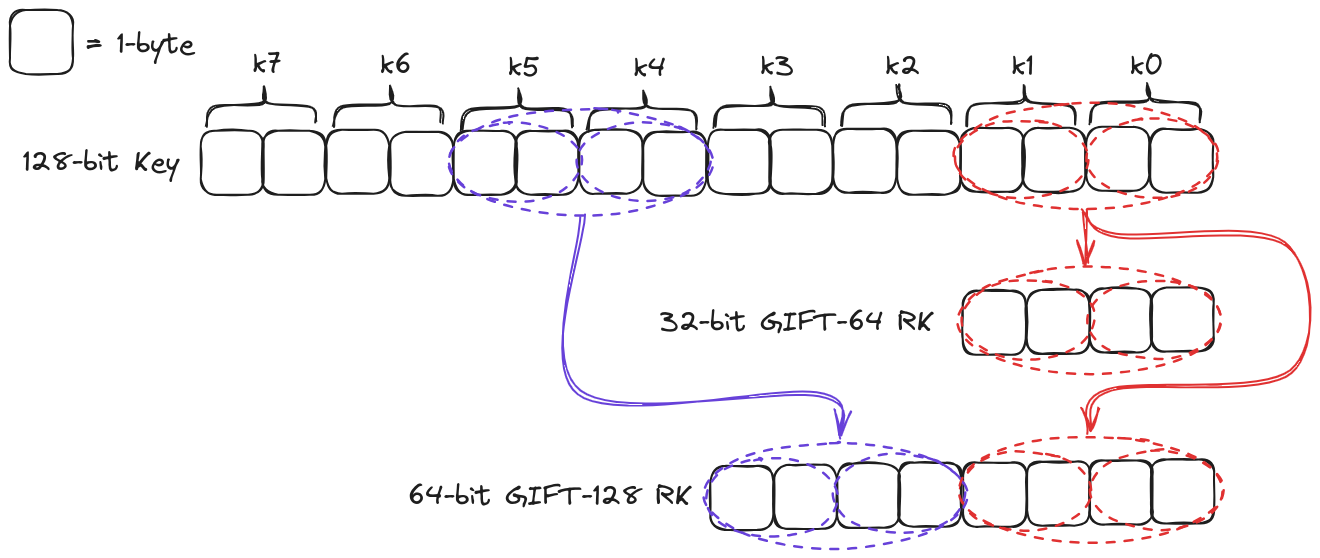
\includegraphics[scale=.3]{image/key_schedule1.png}
\end{figure}

\begin{figure}[h!]\centering
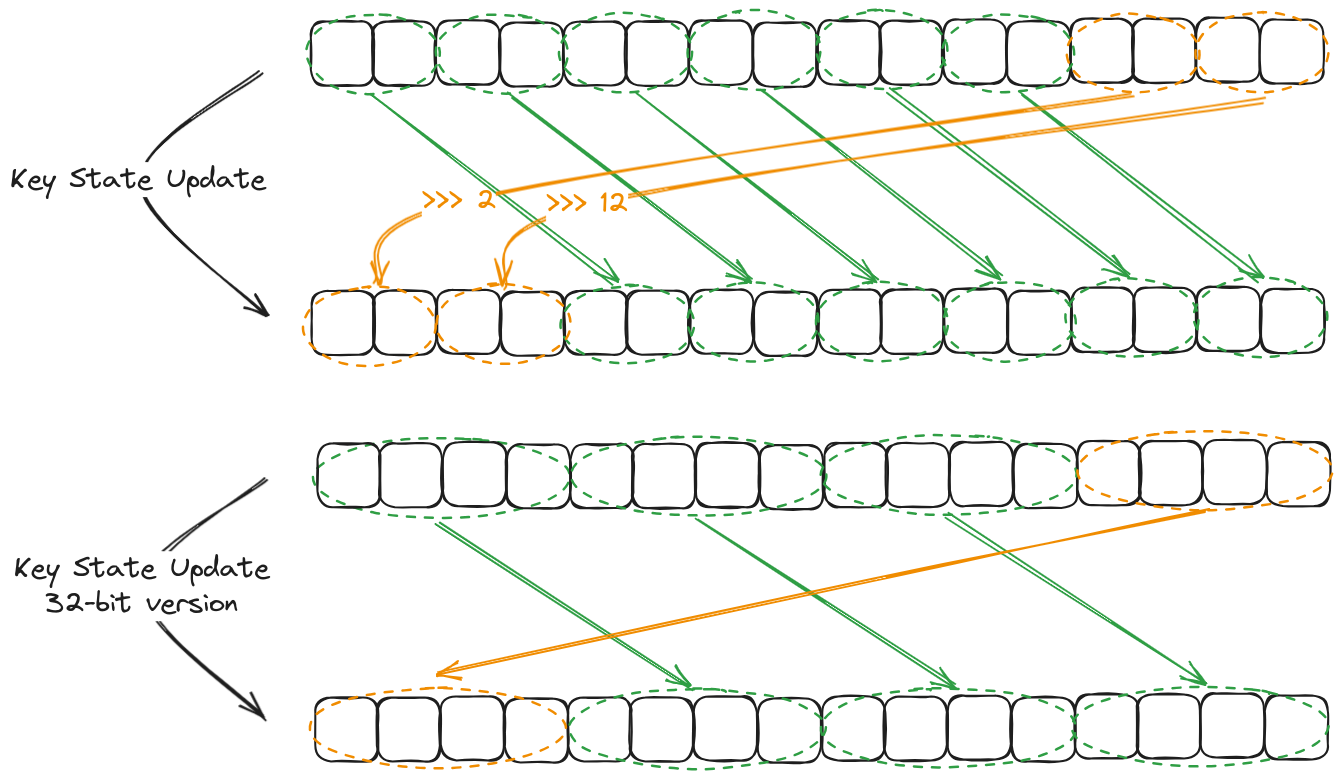
\includegraphics[scale=.3]{image/key_schedule2.png}
\end{figure}
          
\begin{table}[h]\centering\renewcommand{\arraystretch}{1.25}
\centering{\ttfamily
\begin{tabular}{c||c}
	\toprule[1.5pt]
	\textnormal{\bf Rounds} & \textnormal{\bf Constants} \\
	\hline
	\textnormal{\bf 1 - 16} & 01, 03, 07, 0F, 1F, 3E, 3D, 3B, 
	37, 2F, 1E, 3C, 39, 33, 27, 0E \\
	\textnormal{\bf 17 - 32} & 1D, 3A, 35, 2B, 16, 2C, 18, 30, 
	21, 02, 05, 0B, 17, 2E, 1C, 38 \\
	\textnormal{\bf 33 - 48} & 31, 23, 06, 0D, 1B, 36, 2D, 1A, 
	34, 29, 12, 24, 08, 11, 22, 04 \\
	\bottomrule[1.5pt]
\end{tabular}}
\caption{Round Constants generated by 6-bit affine LFSR}
\label{table:round-constants}
\end{table}

\begin{lstlisting}[style=C]
const u8 rCon[48] = {
	0x01U, 0x03U, 0x07U, 0x0FU, 0x1FU, 0x3EU, 0x3DU, 0x3BU,
	0x37U, 0x2FU, 0x1EU, 0x3CU, 0x39U, 0x33U, 0x27U, 0x0EU, 
	0x1DU, 0x3AU, 0x35U, 0x2BU, 0x16U, 0x2CU, 0x18U, 0x30U,
	0x21U, 0x02U, 0x05U, 0x0BU, 0x17U, 0x2EU, 0x1CU, 0x38U, 
	0x31U, 0x23U, 0x06U, 0x0DU, 0x1BU, 0x36U, 0x2DU, 0x1AU,
	0x34U, 0x29U, 0x12U, 0x24U, 0x08U, 0x11U, 0x22U, 0x04U
};
\end{lstlisting}

\newpage
\section{The Round Function}

\subsection{SubCells}

\begin{table}[h]
	\centering{\ttfamily
	\begin{tabular}{|c||cccccccccccccccc|}
		\hline
		$x$     & 0 & 1 & 2 & 3 & 4 & 5 & 6 & 7 & 8 & 9 & a & b & c & d & e & f \\ \hline
		$GS(x)$ & 1 & a & 4 & c & 6 & f & 3 & 9 & 2 & d & b & 7 & 5 & 0 & 8 & e \\ \hline
	\end{tabular}}
	\caption{Specifications of $\gift$ Sbox $GS$}
	\label{table:gift-sbox}
\end{table}
\begin{lstlisting}[style=C]
const u8 GS[16] = {
	0x1U, 0xAU, 0x4U, 0xCU, 0x6U, 0xFU, 0x3U, 0x9U,
	0x2U, 0xDU, 0xBU, 0x7U, 0x5U, 0x0U, 0x8U, 0xEU
};

const u8 invGS[16] = {
	0xDU, 0x0U, 0x8U, 0x6U, 0x2U, 0xCU, 0x4U, 0xBU,
	0xEU, 0x7U, 0x1U, 0xAU, 0x3U, 0x9U, 0xFU, 0x5U
};
\end{lstlisting}


\subsection{PermBits}
The permutation can be expressed as: \[
P_{64}(i)=4\cdot\floor*{\frac{i}{16}}+16\cdot\left[\left(3\cdot\floor*{\frac{i\bmod 16}{4}}+(i\bmod 4)\right)\bmod 4\right] + (i\bmod 4).
\]

\[
x_{P(i)}\gets x_i
\] for $i\in\set{0,\dots,n-1}$.
\vspace{8pt}
\begin{lstlisting}[style=C]
for (u8 i = 0; i < 64; i++) {
	permBits[i] =
		4 * (i / 16) +
		16 * ((3 * ((i % 16) / 4) + (i % 4)) % 4) +
		(i % 4);
}
\end{lstlisting}
\begin{table}[h]
	\centering{\ttfamily
		\begin{tabular}{c||cccccccccccccccc}
			\noalign{\hrule height 1.5pt} % Thick line
			$i$     & 0 & 1 & 2 & 3 & 4 & 5 & 6 & 7 & 8 & 9 & 10 & 11 & 12 & 13 & 14 & 15 \\ \hline
			$P_{64}(i)$ & 0 & 17 & 34 & 51 & 48 & 1 & 18 & 35 & 32 & 49 & 2 & 19 & 16 & 33 & 50 & 3 \\ \noalign{\hrule height 1.5pt} % Thick line
			$i$     & 16 & 17 & 18 & 19 & 20 & 21 & 22 & 23 & 24 & 25 & 26 & 27 & 28 & 29 & 30 & 31 \\ \hline
			$P_{64}(i)$ & 4 & 21 & 38 & 55 & 52 & 5 & 22 & 39 & 36 & 53 & 6 & 23 & 20 & 37 & 54 & 7 \\\noalign{\hrule height 1.5pt} % Thick line
			$i$     & 32 & 33 & 34 & 35 & 36 & 37 & 38 & 39 & 40 & 41 & 42 & 43 & 44 & 45 & 46 & 47 \\ \hline
			$P_{64}(i)$ & 8 & 25 & 42 & 59 & 56 & 9 & 26 & 43 & 40 & 57 & 10 & 27 & 24 & 41 & 58 & 11 \\\noalign{\hrule height 1.5pt} % Thick line
			$i$     & 48 & 49 & 50 & 51 & 52 & 53 & 54 & 55 & 56 & 57 & 58 & 59 & 60 & 61 & 62 & 63 \\ \hline
			$P_{64}(i)$ & 12 & 29 & 46 & 63 & 60 & 13 & 30 & 47 & 44 & 61 & 14 & 31 & 28 & 45 & 62 & 15 \\ \noalign{\hrule height 1.5pt} % Thick line
	\end{tabular}}
	\caption{Specifications of $\gift$-$64$ Bit Permutation}
	\label{table:gift-64-permbit}
\end{table}

\begin{lstlisting}[style=C]
const u8 permBits[64] = {
	0x00U, 0x11U, 0x22U, 0x33U, 0x30U, 0x01U, 0x12U, 0x23U, 
	0x20U, 0x31U, 0x02U, 0x13U, 0x10U, 0x21U, 0x32U, 0x03U, 
	0x04U, 0x15U, 0x26U, 0x37U, 0x34U, 0x05U, 0x16U, 0x27U, 
	0x24U, 0x35U, 0x06U, 0x17U, 0x14U, 0x25U, 0x36U, 0x07U, 
	0x08U, 0x19U, 0x2AU, 0x3BU, 0x38U, 0x09U, 0x1AU, 0x2BU, 
	0x28U, 0x39U, 0x0AU, 0x1BU, 0x18U, 0x29U, 0x3AU, 0x0BU, 
	0x0CU, 0x1DU, 0x2EU, 0x3FU, 0x3CU, 0x0DU, 0x1EU, 0x2FU, 
	0x2CU, 0x3DU, 0x0EU, 0x1FU, 0x1CU, 0x2DU, 0x3EU, 0x0FU
};

const u8 invPermBits[64] = {
	0x00U, 0x05U, 0x0AU, 0x0FU, 0x10U, 0x15U, 0x1AU, 0x1FU, 
	0x20U, 0x25U, 0x2AU, 0x2FU, 0x30U, 0x35U, 0x3AU, 0x3FU, 
	0x0CU, 0x01U, 0x06U, 0x0BU, 0x1CU, 0x11U, 0x16U, 0x1BU, 
	0x2CU, 0x21U, 0x26U, 0x2BU, 0x3CU, 0x31U, 0x36U, 0x3BU, 
	0x08U, 0x0DU, 0x02U, 0x07U, 0x18U, 0x1DU, 0x12U, 0x17U, 
	0x28U, 0x2DU, 0x22U, 0x27U, 0x38U, 0x3DU, 0x32U, 0x37U, 
	0x04U, 0x09U, 0x0EU, 0x03U, 0x14U, 0x19U, 0x1EU, 0x13U, 
	0x24U, 0x29U, 0x2EU, 0x23U, 0x34U, 0x39U, 0x3EU, 0x33U
};
\end{lstlisting}

\subsection{AddRoundKey}

\begin{figure}[h!]\centering
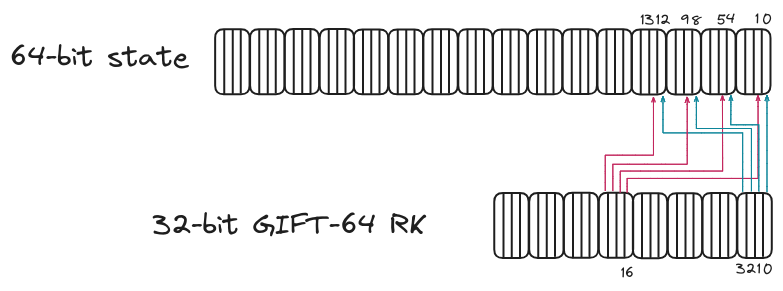
\includegraphics[scale=.6]{image/round_fn.png}
\end{figure}
